\section{Methods}\label{sec:methods}
\subsection{State, information and threat model}
Let $x_t=(q_1,q_2,\dot q_1,\dot q_2)$ be the physical state and $x_t^0$ the state of the same plant under the complete approved command history without corruption. The monitor observes $y_t=x_t+n_t$ and approved position/velocity commands $u_t$. Its maintained state comprises predicted-state and command histories, residual buffers, an alarm bit and a return counter. The evaluator alone receives $x_t$, $x_t^0$ and the corruption schedule. Figure~\ref{fig:model} shows this information boundary.

The attacker changes commands delivered downstream of a protected command copy. Clean commissioning data, the first 100 initialization observations and that copy are trusted. Measurements contain noise, but adversarial sensor forgery is outside this experiment. Once initialized, the protected reference consumes no new measured state. This prevents corrupted motion from changing its predicted history or fitted parameters. It is conditional on the protected inputs, and does not address compromise of both commands and telemetry.

The reference estimates the response to approved commands, initialized from the clean prefix and synchronized through command timing. It is an empirical motion reference, without online parameter adaptation or validated industrial physical fidelity.

\begin{figure*}[t]
\centering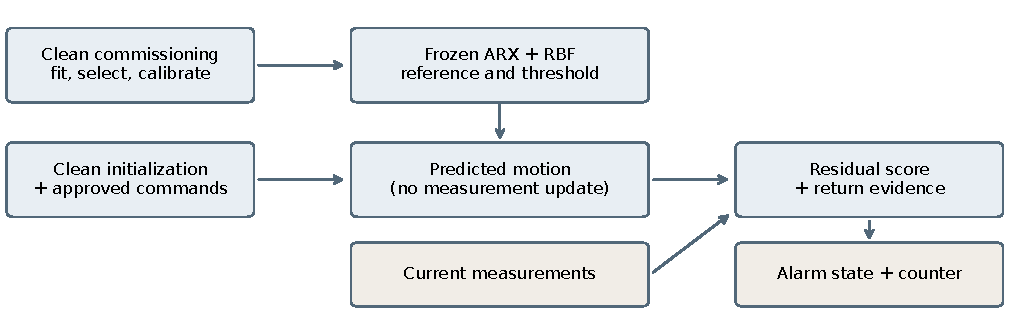
\includegraphics[width=0.82\textwidth]{figures/model.pdf}
\caption{Tested reference and alarm model. Clean data determine the frozen recurrence, correction and threshold. Approved commands drive the reference after initialization. Measurements determine residuals and alarm state, without updating the reference. Counterfactual physical return is restricted to evaluation.}\label{fig:model}
\end{figure*}

\subsection{Stable command-driven reference}
The base is a clean-data autoregressive model with exogenous inputs (ARX). In its fitted coordinates,
\begin{align}
 b_t&=a+\sum_{k=1}^{p}A_k b_{t-k}+\sum_{k=1}^{p}B_k u_{t-k},\label{eq:base}\\
 r_t^0&=\mu+s\odot b_t .
\end{align}
Commands retain their recorded physical coordinates. Training supplies state location $\mu$ and positive scales $s$; constant or nonfinite state channels are rejected. After initialization, Equation~\ref{eq:base} uses predicted states in its own history. The plant-specific orders are 8, 16 and 32 for Q1--Q3, and each selected companion matrix has spectral radius below one. Stability concerns this fitted linear recurrence; it does not establish bounded physical error under arbitrary commands or guarantee transfer to a different robot.

The following control instead uses measured history to predict the next observation. This changes the reference target while retaining the available channels.

\subsection{Training-only residual correction}
A correction estimates systematic normal residuals without feeding them back into the ARX recurrence. Its feature vector is
\begin{align}
 f_t&=[r_t^0,u_{t-1},u_{t-4},u_{t-16},u_{t-32}],\\
 z_t&=(f_t-\mu_f)/s_f,\label{eq:features}
\end{align}
with 20 dimensions. The feature means and scales use training observations only; a feature scale at or below $10^{-12}$ is replaced by one. This is distinct from rejecting a constant physical-state scale. Farthest-point selection in standardized training space deterministically chooses $K$ centers $c_i$, starting from the observation closest to the origin. The bandwidth $h$ equals a selected multiplier times the median positive center distance.

The radial basis functions (RBFs) and corrected output are
\begin{align}
 \phi_i(z)&=\exp\{-\|z-c_i\|_2^2/(2h^2)\},\\
 r_t&=r_t^0+s\odot W^T[\phi_1(z_t),\ldots,\phi_K(z_t),1]^T.\label{eq:rbf}
\end{align}
The four-output coefficient matrix minimizes
\begin{equation}
 N^{-1}\|\Phi W-E\|_F^2+\lambda\|W_{1:K,:}\|_F^2,\label{eq:fit}
\end{equation}
where $E$ contains standardized clean residuals. The intercept is unpenalized, and nonfinite fits are rejected. A linear correction uses the same 20 standardized features and objective, providing a direct nonlinearity control. RBF heads contain $4(K+1)$ coefficients: 132 for 32 centers and 260 for 64 centers. These counts exclude stored centers, feature statistics and the base ARX. The linear head contains 84 coefficients.

Bounded activations and fixed weights bound correction magnitude, not physical prediction error. Weights, centers, scales and thresholds remain frozen during evaluation.

\subsection{Entry score and alarm-clearance state}
Define $e_t=(y_t-r_t)/s$ and $a_t=\max_j|e_{t,j}|$. Strict exceedance $a_t>\tau$ raises an alarm and resets its return counter. At other eligible points, the candidate checks
\begin{equation}
 g_t=\mathrm I\!\left\{\|\bar e_t(5)\|_\infty\le0.1\ \land\
 \|\bar e_t(41)\|_\infty\le0.1\right\},\label{eq:gate}
\end{equation}
where $\bar e_t(m)=m^{-1}\sum_{k=0}^{m-1}e_{t-k}$. Ten consecutive qualifying points clear an active alarm; a new entry exceedance has priority. The windows contain 0.10 and 0.82 seconds of samples at 50 Hz, and the dwell contains 0.20 seconds. Entry scoring starts at zero-based index 100 and covers 1,100 points per episode. Clearance uses only residuals from that scored interval: the five-point window first becomes ready at index 104 and the 41-point window at 140. Dual-window clearance can first occur at 149 with ten-point dwell, or at 140 without dwell. Entry remains possible before clearance readiness; these distinct eligibility masks do not shorten the score population. Signed means can cancel oscillatory deviations, so the gate measures agreement with the reference rather than certifying physical return.

The short gate is partly constrained by the entry rule: after five consecutive non-exceedances, the mean residual norm is no greater than the largest of those five scores, hence no greater than $\tau$. The RBF thresholds are 0.03697, 0.03712 and 0.05740, all below 0.1. Thus the short gate passes on those windows. Earlier exceedances can still alter streak timing; this conditional result is not a universal equivalence proof.

Invalid history resets the evidence streak and cannot clear an active alarm; the implemented known-state mask then remains false. The final campaign admits complete finite episodes, so missing-data behavior is software-tested only. Algorithm~\ref{alg:replay} specifies the causal order.

\begin{table*}[t]\centering
\caption{Algorithm 1: normal-only fitting, selection and freezing.}
\label{alg:fit}
\begin{tabular}{>{\raggedright\arraybackslash}p{0.055\textwidth}>{\raggedright\arraybackslash}p{0.88\textwidth}}\toprule
Input & Separate clean training, development and calibration episodes; declared candidate grid and tie-break rule.\\\midrule
1 & Fit training-only state statistics and candidate ARX references; reject invalid or unstable candidates. Preserve each candidate outcome.\\
2 & Generate free-running training predictions from clean initial histories. Construct the 20-dimensional features and fit their statistics and centers on training only.\\
3 & Solve the ridge objectives. Evaluate each frozen candidate on the same normal-development episodes, keeping episode boundaries intact.\\
4 & Within the linear and RBF roles separately, select by worst-episode residual $q_{.99}$, then mean RMSE, coefficient count and identifier. Preserve the chosen artifact without refitting on development.\\
5 & Score the separate normal-calibration population. Set the fixed entry threshold to ascending rank 5,445 of 5,500 scores.\\
6 & Seal models, transforms, thresholds, methods, seeds, inputs, code, budgets and criteria before generating the new evaluation conditions.\\\bottomrule
\end{tabular}
\end{table*}

\begin{table}[t]\centering
\caption{Algorithm 2: prospective monitoring of one episode.}\label{alg:replay}
\begin{tabular}{>{\raggedright\arraybackslash}p{0.12\columnwidth}>{\raggedright\arraybackslash}p{0.76\columnwidth}}\toprule
Input & Frozen model and threshold; clean 100-point prefix; approved commands and current measurements.\\\midrule
1 & Initialize predicted history from the prefix; set alarm, evidence counter and post-prefix residual buffers to zero/empty.\\
2 & Predict $b_t$ from earlier predicted states and commands; compute $r_t$ using the frozen correction.\\
3 & At $t\ge100$, read $y_t$, score and append $e_t$. Before full post-prefix windows exist, entry is allowed but clearance is not. No label or future measurement is read.\\
4 & If history is invalid, reset the streak and retain alarm state. Otherwise, an entry exceedance raises alarm and resets the streak.\\
5 & If alarm is active without an exceedance, increment the streak when $g_t=1$, otherwise reset it. Clear after the declared dwell.\\
6 & Save score, validity and alarm at index $t$. Advance predicted history, leaving fitted parameters fixed. Continue across attack boundaries.\\\bottomrule
\end{tabular}
\end{table}

\subsection{Physical return and uncertainty}
The evaluator measures $d_t=\max_j|x_{t,j}-x_{t,j}^0|/s_j$. Reference/noise bounds $b_t,\eta_t$ would give $d_t\le a_t+b_t+\eta_t$. Sufficient return requires $a_t+b_t+\eta_t\le\delta$, which is infeasible when the allowance exceeds the tolerance. Empirical maxima under Gaussian noise are not deterministic bounds. Appendix~\ref{app:uncertainty} develops this limitation and the window diagnostic.
\subsection{Bounded extension: contextual residual evidence}\label{sec:contextmethod}
The matched replay diagnoses excessive retention of noisy entries, with a smaller concentration of errors around legitimate command steps. We therefore investigate a command-conditioned empirical allowance using the saved base ARX; RBF is not required by this extension. The context state depends only on approved command increments:
\begin{align}
 d^u_t&=\|(u_t-u_{t-1})/s\|_\infty,\\
 h_t&=\max\{d^u_t,\exp(-1/m)h_{t-1}\},\quad h_0=0.
\end{align}
Training 90th/99th context quantiles define three bins. Each bin's width $w_t$ is the ascending 99th-percentile base residual score on separate normal calibration observations, with a global-quantile fallback below 30 observations. Context state evolves causally, but bin boundaries, widths and reference parameters are frozen. The top bin extends beyond the training maximum: this is empirical extrapolation, with context-support frequency reported, not a guaranteed uncertainty set.

Using the instantaneous residual score $a_t$, define
\begin{equation}
 L_t=\max(0,a_t-w_t),\qquad U_t=a_t+w_t.
\end{equation}
The candidate enters when $L_t>0.1$, clears when $U_t\le0.1$, and otherwise retains its previous state. No dwell or residual averaging is added. The unresolved region is reported even when the alarm is inactive. If $w_t$ truly bounded the combined nominal-reference and measurement error in the same standardized infinity norm, triangle inequalities would give $L_t\le d_t\le U_t$. An empirical normal quantile does not establish that bound under attack or plant shift. We test the decision rule as a heuristic, without a coverage or safety theorem.

The finite candidate set uses memories $m=10,40$ samples (0.2/0.8 s). K13 normal episodes fit bin boundaries; L13 normal episodes calibrate widths; M13 normal episodes select by benign alarm points, starts, mean allowance and then memory. These are exposed development data separated by task, not fresh validation. Two memories on each plant give six plant-specific fits across two candidate memory choices; no ARX or RBF weights are refitted. The selected candidate is frozen before new evaluation.

The essential matched control uses identical context and entry decisions but clears at $a_t\le0.1$, isolating the extra width in clearance. Other controls use a constant global width, contextual entry without retention, the physical-tolerance point rule $a_t>0.1$, and a three-of-five original-threshold entry rule, alongside the historical base/RBF and following rules. Input-dependent thresholds, residual intervals and hysteresis already exist~\cite{inputthreshold,motionconformal,interval}; an observed gain would require a specific advantage over these ordinary controls before an originality argument.

